%
% Webapplikation
% Abschlussarbeit (Bachelor)
%
% Thema: Erstellung einer Browser Extension zur Usability Evaluierung von beliebigen Web-Applikationen über Heatmaps.
% Betreuer 1: Prof. Dr. Targo Pavlista
% Betreuer 2: Siamak Haschemi
%
% @author Christian Bromann <contact@christian-bromann.com>
%

\section{Webapplikation}

Die Webapplikation ist die Administrationsoberfläche der gesamten Anwendung. Hier erstellt der User des \textit{thEvaluator} Frameworks die Testcases, passt sie an und wertet sie anschließend aus. Wie es sich für einen administrativen Bereich gehört, sollte dieser passwortgeschützt sein und nur bestimmten Personen Zugang gewähren. Aus zeitlichen Gründen wurde jedoch auf ein User-Management verzichtet. Betritt man die Startseite des Bereiches, so erhält der User eine Übersicht über die bereits angelegten Testcases. Neben dem Namen sind drei Aktionsbuttons zu finden, mit denen man den Testcase bearbeiten, löschen oder dessen Details betrachten kann. Ganz oben neben dem \textit{thEvaluator} Logo befindet sich die Navigation. Diese leitet den Benutzer zum Erstellen oder Evaluieren von Testcases weiter.

\begin{center}
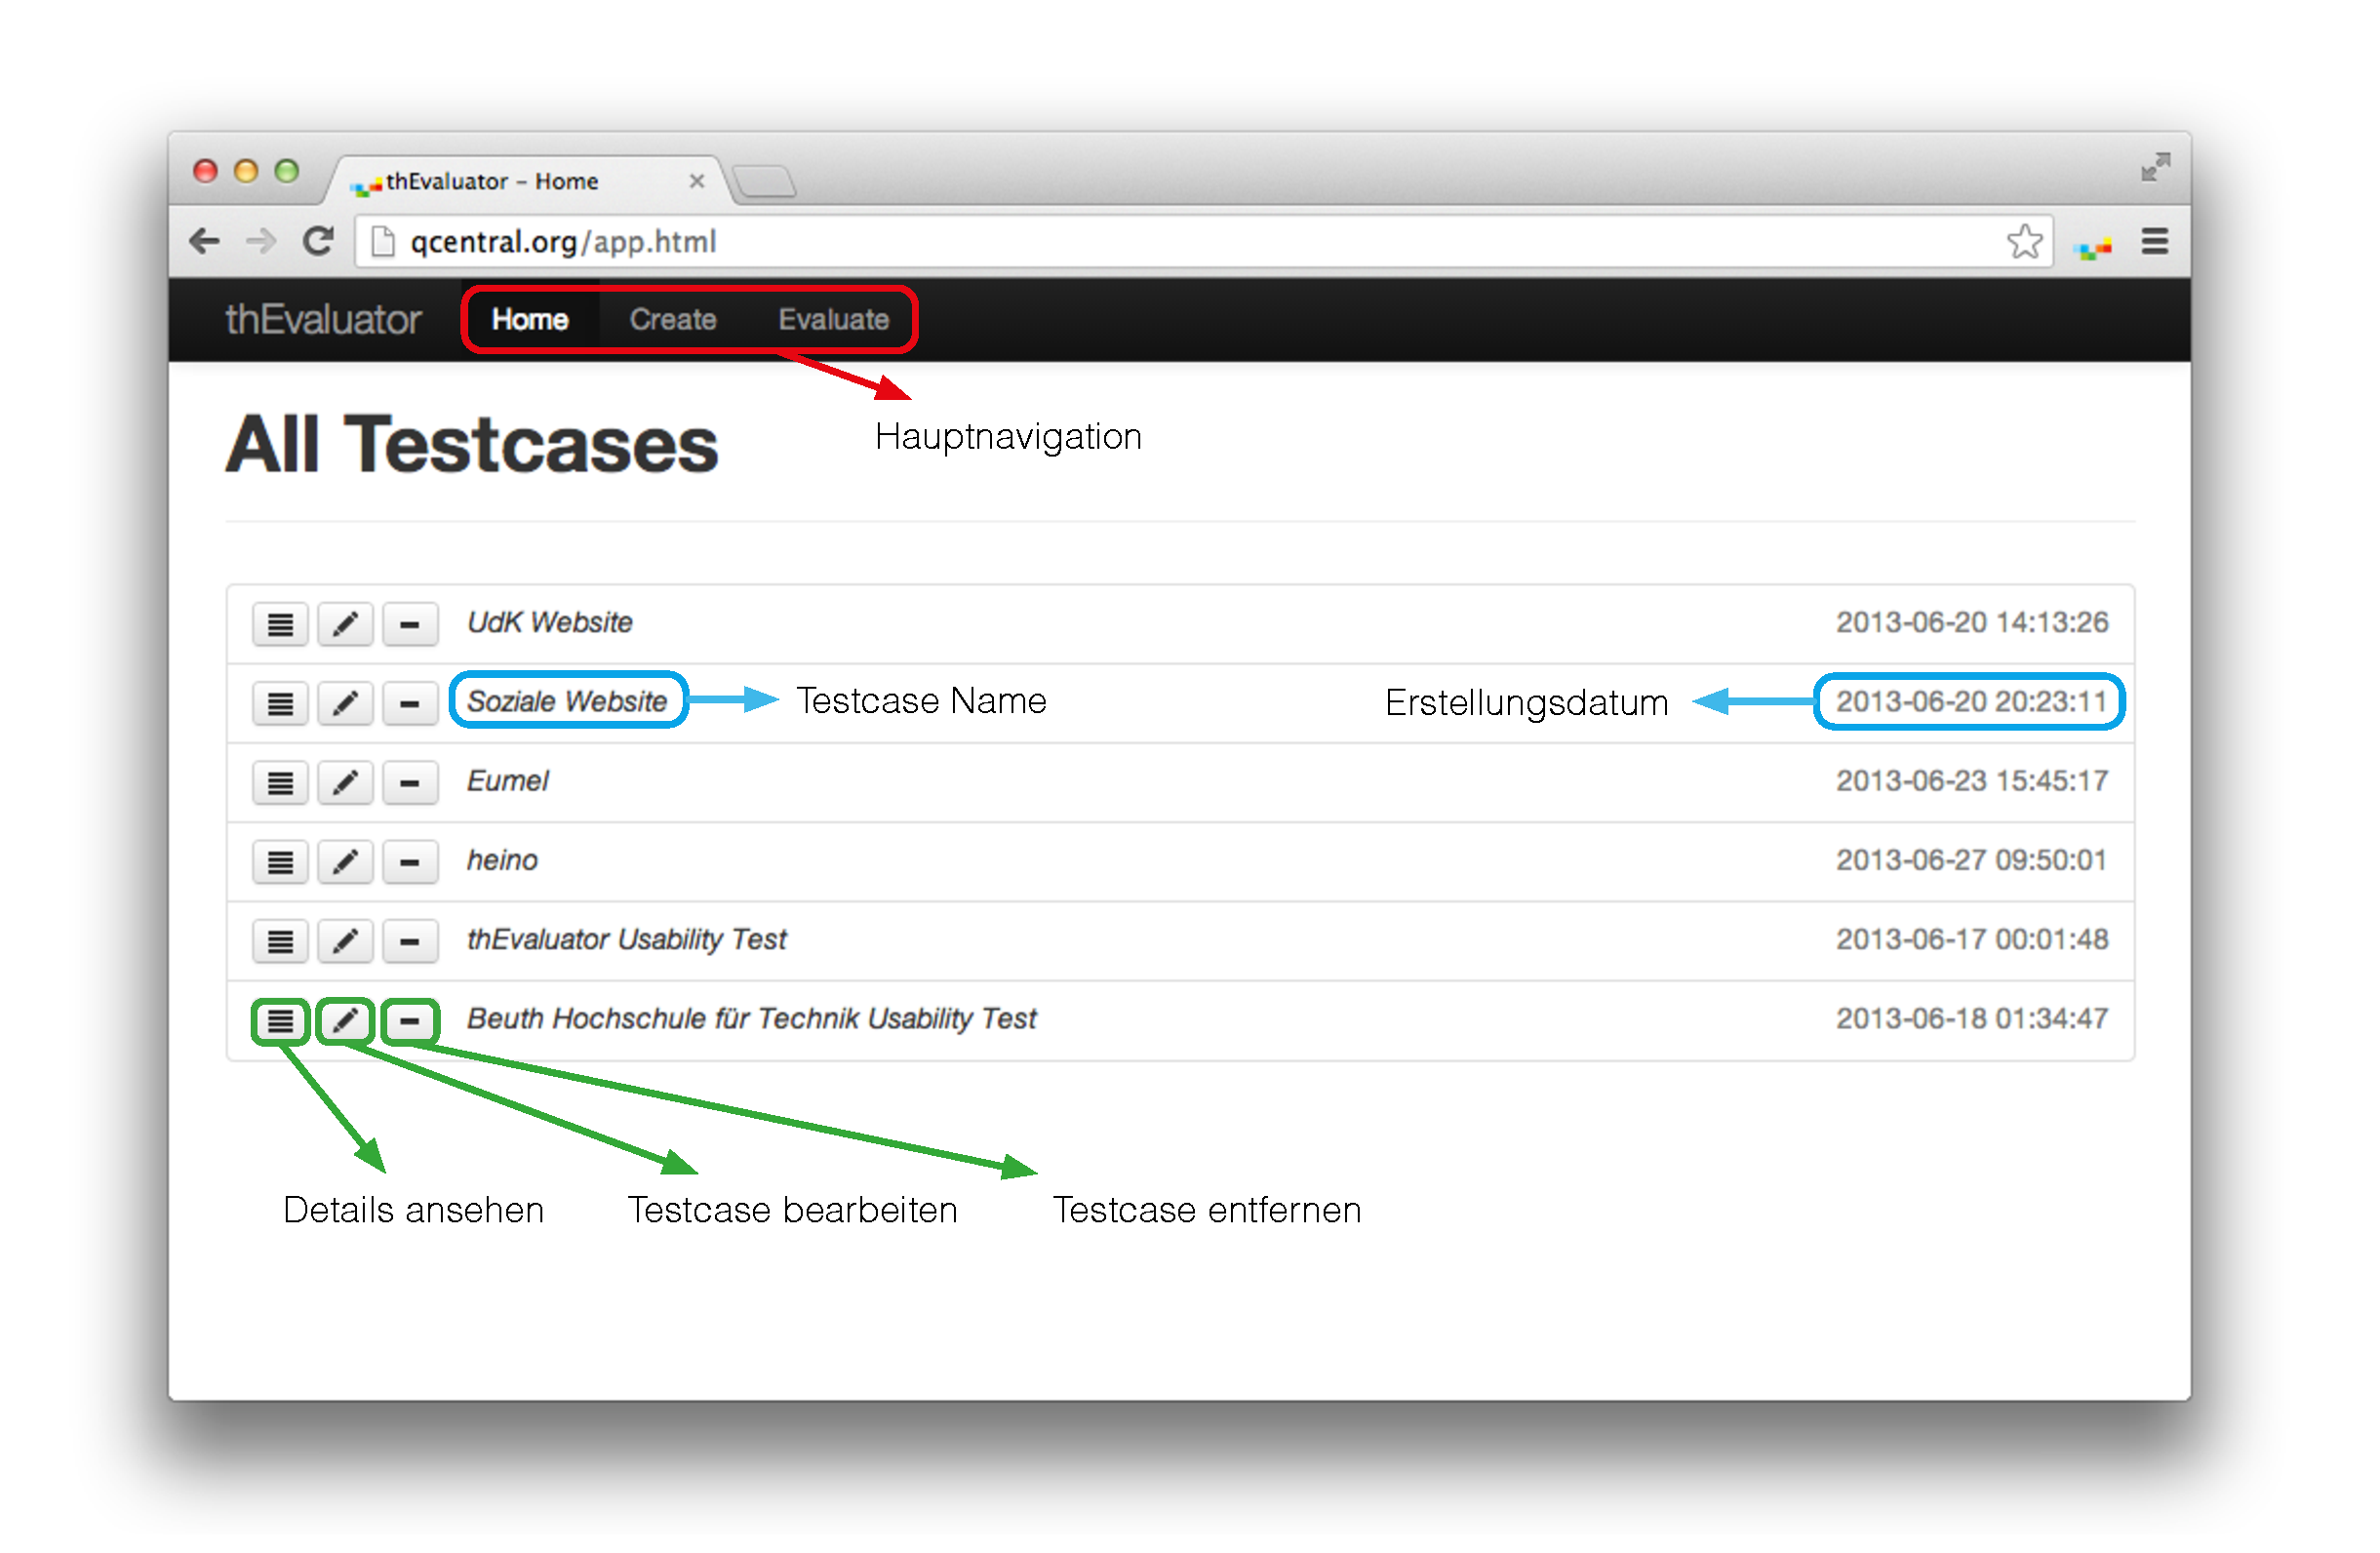
\includegraphics[scale=0.40]{./images/webappscreen}
\end{center}
\begin{figure}[htb]
   \centering
   \caption{Administrationsoberfläche}
    \label{webappview}
\end{figure}

Alles beginnt mit der Erstellung eines Testcases. Es braucht nicht viel Zeit und Eingaben, um einen zu erstellen. Nach dem Klick auf \textit{Create} öffnet sich die Formularansicht. Als erstes vergibt man einen Namen für den Testcase, gefolgt von einer URL. Diese ist der Startpunkt für den Testcase. Es ist dabei nicht notwendig von der Startseite einer Website zu beginnen. Führt man bspw. einen Test für das firmeninterne Intranet durch, so kann auch eine Netzwerk-URL eingegeben werden. Wichtig ist nur, dass die Teilnehmer die notwendigen Rechte zum Zugriff auf die Seite besitzen. Eine weitere wichtige Angabe ist die der Auflösung. Jeder Testcase muss eine feste Auflösung vorschreiben, um die Verhältnisse für jeden Probanden gleich zu setzen. Die Extension verkleinert oder vergrößert beim Starten des Testcases dann automatisch das Browserfenster. Dadurch wird sichergestellt, dass die Testuser unter den gleichen Vorraussetzungen, was Auflösung angeht, die Seite nutzen. Zudem ermöglicht es Usability-Tests für Webseiten mit einem \textit{Responsive Design}. Wählt der User eine Auflösung für mobile Geräte, wie z.B. 320 x 480 px, so erhält er automatisch die Version der Website, die ein mobiler User ebenfalls erhalten würde. Obwohl das Verhalten zwischen Mobil- und Desktop-User dann immer noch nicht das Gleiche ist, bekommt man trotzdem einen recht guten Eindruck davon, wie die mobile Version der Seite genutzt wird.

\begin{center}
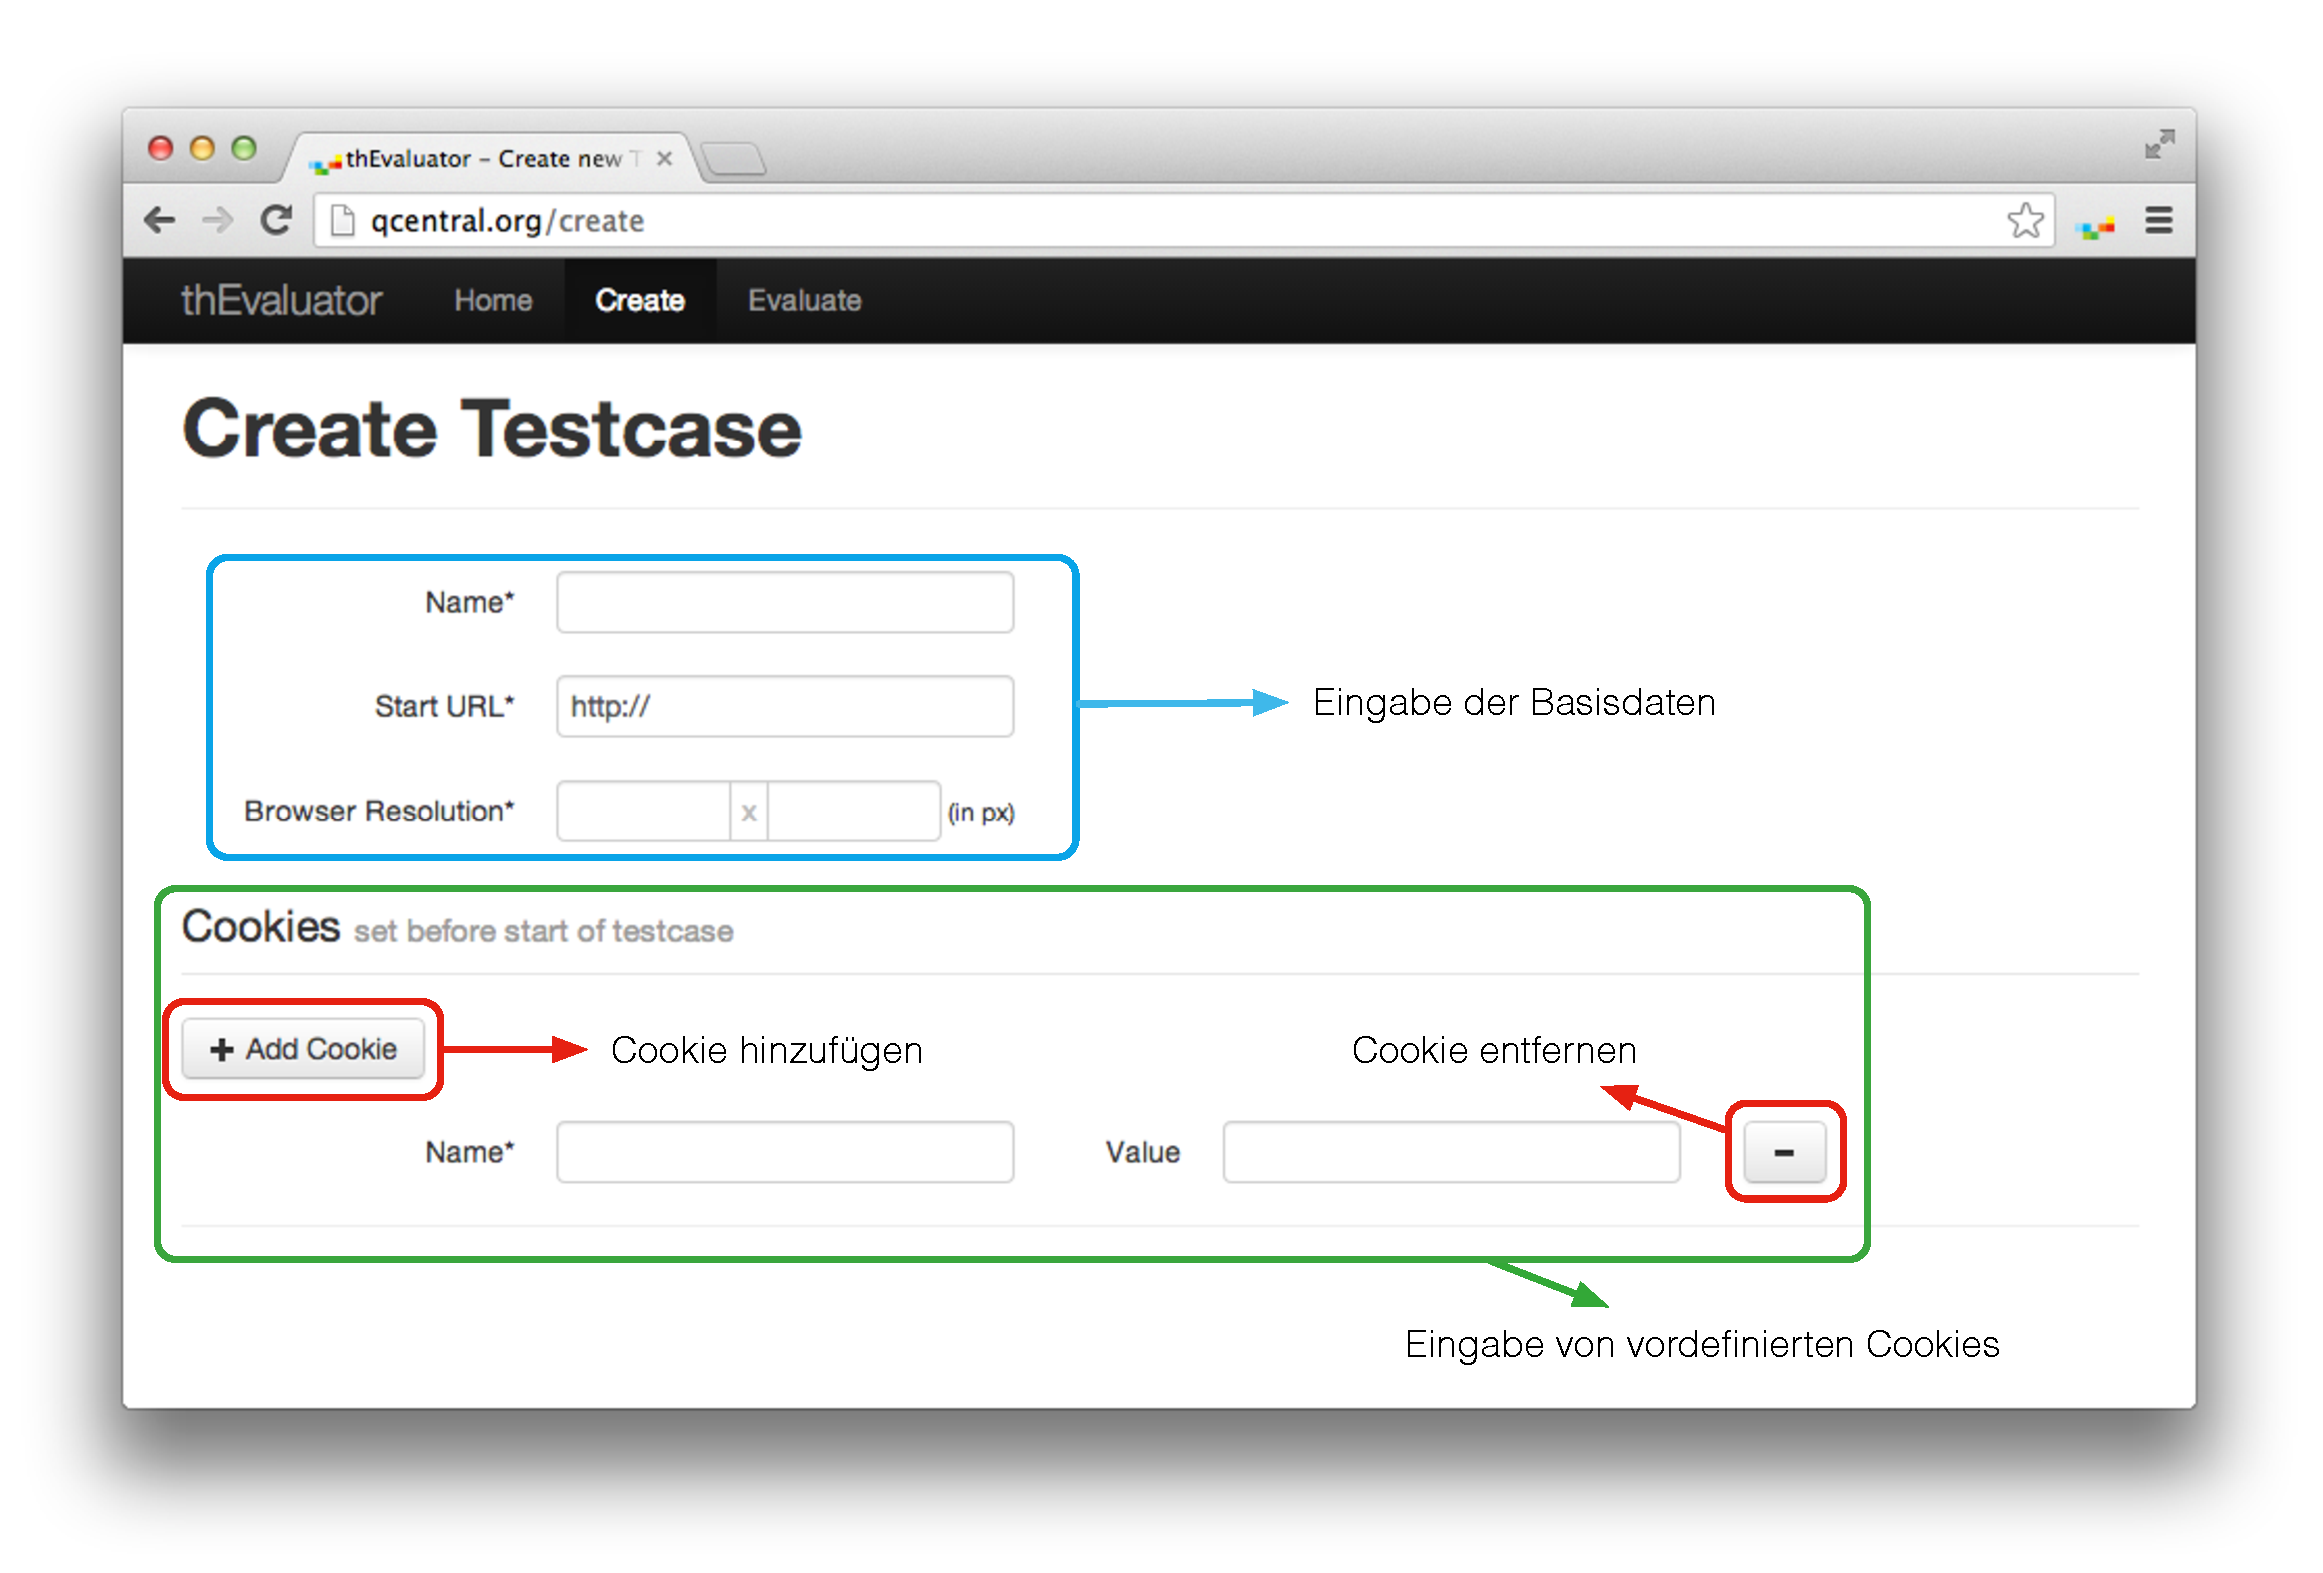
\includegraphics[scale=0.40]{./images/createscreen}
\end{center}
\begin{figure}[htb]
   \centering
   \caption{Formularansicht}
    \label{createview}
\end{figure}

Um den Usability-Test für jeden Bereich einer Webseite möglich zu machen, gibt es zudem die Möglichkeit, Cookies vor dem Start setzen zu lassen. Möchte der User bspw. eine Website testen lassen, die noch nicht veröffentlicht ist, so kann er hier spezielle Cookies definieren, die die Seite erkennt und den Zutritt darauf gewährt. Die Extension setzt diese Cookies vor Beginn des Testcases für alle Subdomains und Pfade der Website. Als letztes werden die Tasks definiert. Diese enthalten, neben dem Namen und einer Aufgabenbeschreibung, ein \textit{required} Feld, welches angibt, ob der Testcase beendet ist, wenn der Proband die Aufgabe nicht lösen kann. Dadurch ist es möglich, eine Aufgabe, wie z.B. die Auswahl eines Produktes im Online-Shop, als Vorraussetzung für die Folgeaufgaben, z.B. die Ware in den Warenkorb zu packen, auszuwählen.

\begin{center}
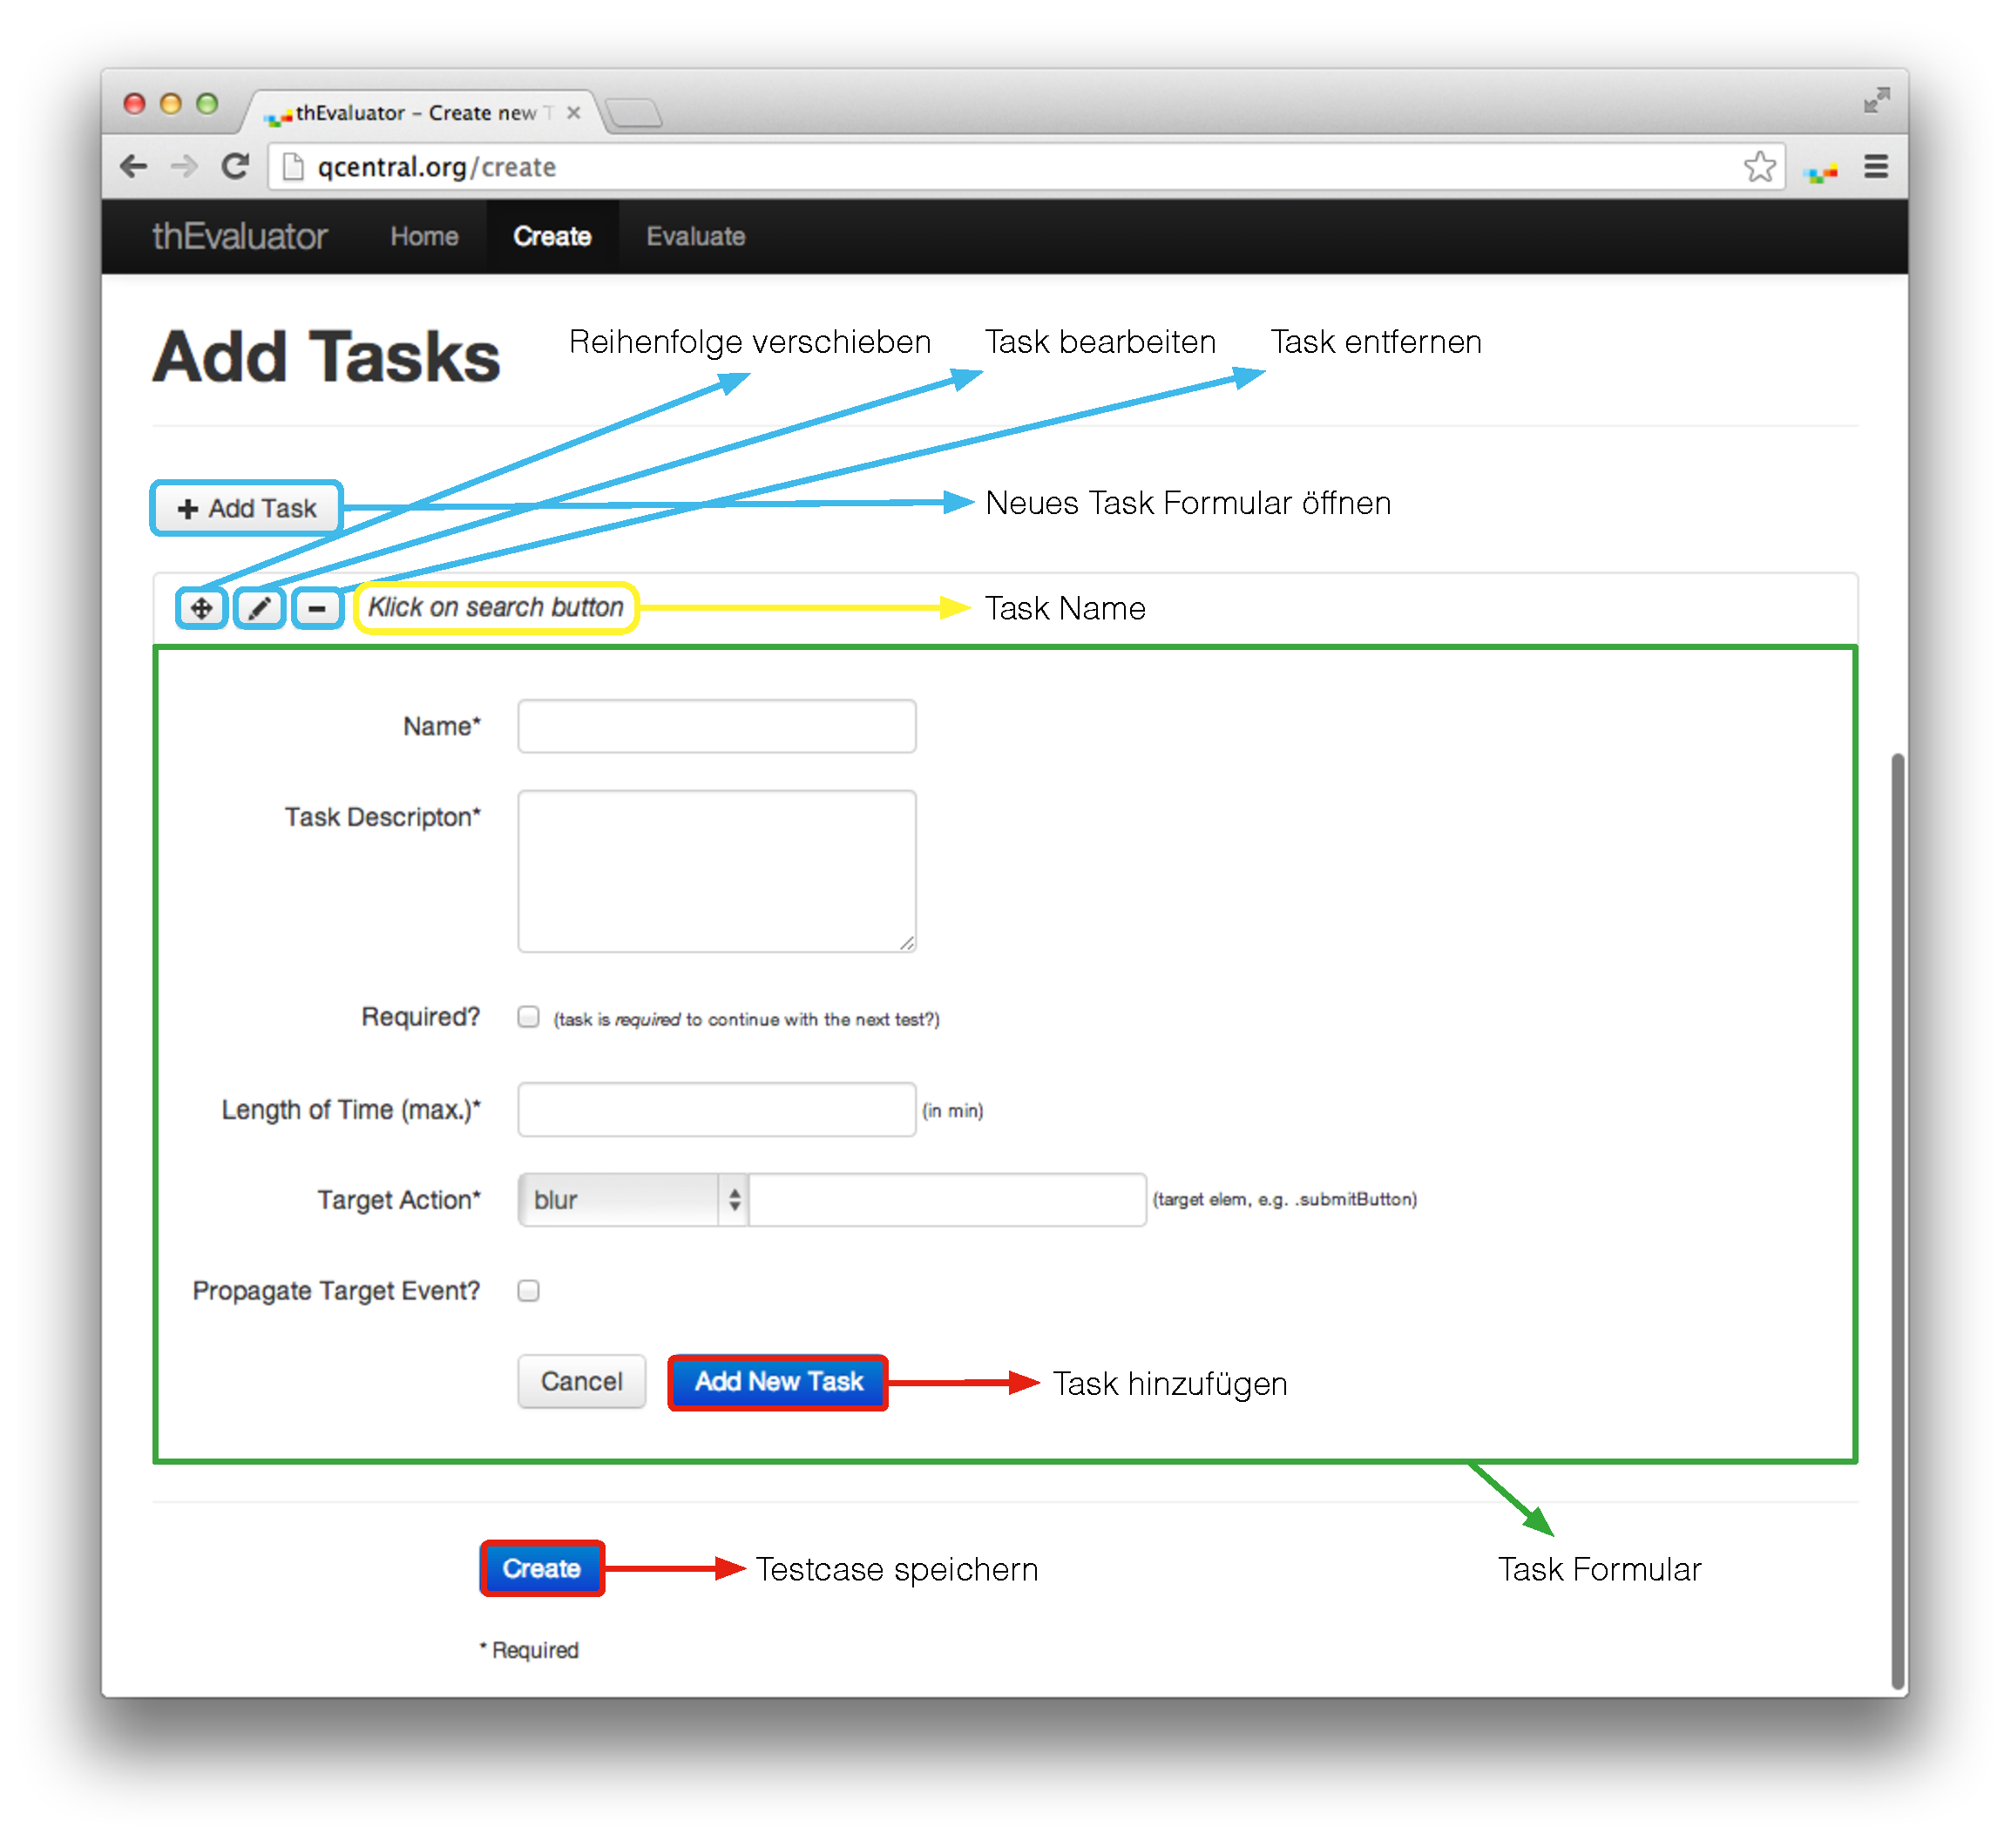
\includegraphics[scale=0.4]{./images/taskscreen}
\end{center}
\begin{figure}[htb]
   \centering
   \caption{Task-Formular}
    \label{taskscreen}
\end{figure}

Ein weiteres Attribut eines Tasks ist die Zeit. Die Aufgabe kann als gescheitert angesehen werden, wenn der Proband zu lange zum Lösen dieser benötigt. In einem realen Szenario würde der User eine Website verlassen, wenn er nach einer bestimmten Zeit nicht an sein Ziel findet. Als nächstes folgt die Angabe des Ziel Events. Dieses besteht, wie in Kapitel \ref{events} beschrieben, besteht dieses aus einer Action und einem Element aus dem DOM. Möchte man bspw. den Klick auf einem Link mit einer bestimmten URL als Ziel einer Aufgabe definieren, so wählt man eine \textit{click}-Action auf einem Element mit dem Selektor \textit{a[href=''\textbf{ URL }'']}. Es kann auf alle CSS3 Selektoren zurückgegriffen werden. Dies macht die Einschränkung der Elemente sehr flexibel. Als letztes ist die Angabe des \textit{Propagation} Attributes möglich. Dies setzt fest, ob das Event, wie z.B. der Klick nach dem Abfangen durch die Extension abgefangen werden soll oder nicht. Bleiben wir beim Beispiel mit dem Klick auf einen Link, so würde sich die neue Seite nur öffnen, wenn die Checkbox aktiviert ist. Der User würde dann mit dem nächsten Task auf dieser Seite weiter machen. Ist die Box nicht aktiviert, so verbleibt er auf der Seite, da die Extension den Klick abfängt, bevor der Browser den Befehl zum Öffnen der neuen Seite bekommt.\\
\\
Nachdem ein paar Aufgaben für den Testcase erstellt wurden, ist im Nachhinein noch möglich, jeden einzelnen Task zu bearbeiten. Zudem kann die Reihenfolge der Aufgaben via Drag\&Drop verschoben werden (siehe \glqq Reihenfolge verschieben\grqq{}-Button in Abbildung \ref{taskscreen}). Als letztes wird der Testcase gespeichert und erhält eine 10-stellige ID, die allen Probanden geschickt werden kann, die an dem Test teilnehmen. Zum Schluss können die Ergebnisse auf der \textit{Evaluate} Seite (siehe Hauptnavigation) ausgewertet. Näheres dazu wird in Kapitel \ref{evaluation} erläutert.


\subsection{Aufbau}

Die Webapplikation des \textit{thEvaluator} Frameworks ist mit den modernsten Frontend-Web-Technologien dieser Zeit entwickelt wurden. Es bedient sich, ebenso wie die Extension-Komponente, dem Grunt Tool für Buildprozesse und Entwicklungsworkflows und nutzt mit Bower\footnote{\url{http://bower.io}} ein Package Manager für das Dependancy-Management. Bereitgestellt wird dieses Set an Tools durch Yeoman\footnote{\url{http://yeoman.io}}. Dieses konfiguriert Grunt und Bower zu einem in sich harmonierenden Workflow und bietet für die Entwicklung verschiedene Scaffolding Möglichkeiten an. Entwickelt wurde dieses System von den erfahrensten Webentwicklern dieser Zeit und einer großen Community, die ständig neue Tools zur Erstellung besserer Webapplikationen entwickelt.\\
\\
Für das Deployment werden verschiedene Dependencies vorausgesetzt. Das System benötigt \textit{Node}, \textit{Ruby} und \textit{Sass\footnote{\url{http://sass-lang.com/}}}. Letztere werden zur Kompilierung der CSS Dateien benötigt. Die Webapplikation nutzt den CSS-Preprozessor Sass, um verschiedene Features, wie z.B. Vererbung oder Verschachtelung der CSS Regeln, nutzen zu können. Das Design baut auf dem bekannten \textit{Twitter-Bootstrap\footnote{\url{http://twitter.github.io/bootstrap/}}} auf und erhält damit ein elegantes Grunddesign, welches flexibel genutzt werden kann. Da die Webapplikation lediglich ein Prototyp ist, wurde auf die Erstellung eines eigenen Designs verzichtet, um die Entwicklung zu beschleunigen. Nachdem auf dem System die Grund-Dependencies installiert sind, müssen Grunt und Bower auf dem System heruntergeladen und eingerichtet werden. Der Parameter \textit{-g} gibt an, dass diese Pakete global auf dem System installiert werden und dadurch einen Befehl für das Kommandozeilentool bereitstellen.

\vspace{1cm}
\begin{lstlisting}[caption=Installation von Grunt und Bower auf dem System,label=installPackages]
$ [sudo] npm install grunt -g
$ [sudo] npm install bower -g
\end{lstlisting}
\vspace{1cm}

Bower ist wie NPM eine Package- und Dependancy-Manager. Jegliche Zusatzkomponenten, wie z.B. jQuery oder Backbone, die die Webapplikation für den Frontend-Bereich benötigt, werden in einer zentralen Datei mit einer festdefinierten Versionsnummer festgehalten und können bequem über die Konsole heruntergeladen werden. Dies erspart dem Entwickler den Aufwand die Datei manuell herunterzuladen. Die \textit{thEvaluator}-Webapplikation benötigt für verschiedene Teile der Anwendung Zusatzbibliotheken. Diese werden im Frontend-Bereich im JavaScript oder auf System-Ebene für die Build-Prozesse benötigt. Listing \ref{installDependencies} zeigt, wie jegliche benötigte Bibliotheken herunterzuladen werden müssen.

\vspace{1cm}
\begin{lstlisting}[caption=Installation der Zusatzbibliotheken für die Webapplikation,label=installDependencies]
$ npm install
$ bower install
\end{lstlisting}
\vspace{1cm}

Bevor nun die Applikation genutzt werden kann, müssen die Dateien deployt werden. Im Gegensatz zu Java, bei denen dabei binäre Dateien erzeugt werden, wird bei einem Deployment einer Webapplikation Dateien zusammengefügt und minifiziert. zum Einen werden jegliche Templates, JavaScripte und Bibliotheken in eine Datei zusammengefasst und minifiziert. Zusätzlich werden die Sass Dateien zu CSS Dateien übersetzt und Bilder optimiert. Der Gesamte Vorgang dauert ca. 10min und resultiert mit einem \textit{dist}-Ordner, in dem die alle präparierten Dateien zusammengefügt liegen. Als Letztes muss lediglich eine Serverinstanz erstellt werden, die die Dateien ausliefert. Dies wird dank Yeoman in einem Grunt-Task bereits geliefert. Die Webapplikation nutzt, genauso wie die API, einen \textit{forever}-Prozess, um diese Serverinstanz dauerhaft am laufen zu halten. Listing \ref{build} zeigt, die Befehle, die den Deploymentprozess anstoßen und die App starten.

\vspace{1cm}
\begin{lstlisting}[caption=Deployment und Start der Webapplikation,label=build]
$ grunt build
$ grunt forever:start
\end{lstlisting}
\vspace{1cm}

\subsection{Architektur}
% Backbone, Models (die DB Modelle abbilden) Collections, Views
% MV* ErklŠärung

\subsection{Evaluation}
\label{evaluation}
% Was ist mšglich, wie weit gehen die Auswertungen

\subsection{Aufbereitung}
% wann werden welche Daten geladen (lazy loading)
% handling der Datenmenge

\subsection{Auswertung}
% Walkpath map: cognitives model: "journal of emerging technologies"
% welche Auswertungswidgets gibt es / Bedeutung
% bei der Erklärung des walkpath widgets, dies mit einbauen
% Die Analyse von Verhaltens- und Navigationsmustern und der anschließenden Verbesserung der Link Struktur einer Seite fällt unter den Begriff des \textit{Web-Usage-Mining}, welches ein Untersuchungsgegenstand des \textit{Web Minings} ist. \cite{webusagemining}. Auf Grundlage dieser Navigationsmuster lassen sich Pfade herleiten und Linkstrukturen berechnen. Wissenschaftler aus China haben daraus eine neuartige Methode entwickelt, die Qualität der Linkstruktur mathematisch zu berechnen \cite{linkStructure}.\\
% \\
% Es wird davon ausgegangen, dass die Link Struktur einer Seite durch \textbf{G} in \ref{structure} als gewichtet-direkterer Graph repräsentiert wird.
% 
% \begin{equation}
%     G = (N, P, L, W)
%     \label{structure}
% \end{equation}
% 
% \begin{itemize}
%     \item N =  Anzahl der Seiten einer Website (Anzahl der Knoten des Graphen)
%     \item P = Menge aller Knoten in G, $ \{P_i | i \in [1,N]\} $
%     \item L = Menge aller Kanten in G, $ \{L_{i,j} | i \neq j; i,j \in [1,N]\} $\\
%     	     ($ L_{i,j} $ entspricht dabei ein Link von $ P_i $ zu $ P_j $)
%     \item W = Menge aller Knoten-Gewichtungen in G, $\{W_{i,j} | i \neq j; i,j \in [1,N]\}$\\
%              \\
%              Die Wahrscheinlichkeit dafür, das der Besucher auf der Seite $P_i$ einen % Link $L_{i,j}$ folgt und dadurch auf $P_j$ gelangt wird
%              durch $W_{i,j}$ gekennzeichnet und berechnet sich wie folgt:\\
%              \\
%              $W_{i,j} = \frac{V_{i,j}}{ \sum_{k = 1}^{D_i} V_{idk}}$\\
%              \\
%              $D_i$ ist definiert als Menge aller Seiten, die auf $P_i$ durch Links erreichbar sind.\\
%              $V_{i,j}$ wird dadurch zum Bogenmaß der Kante von $P_i$ zu $P_j$
% \end{itemize}

% wann kann man mšögliche Resultate ableiten